\documentclass{article}
\usepackage[utf8]{inputenc}
\usepackage{amsfonts} 


\title{Robustness of Gaussian Process}
\author{Shiyu Zhang }
\date{}

\usepackage{natbib}
\usepackage{graphicx}

\begin{document}

\maketitle

\section{Introduction}
In this paper, our goal is to study the relationship between an input random variable $X \in \mathbb{R}^d$  and the corresponding output random variable $Y \in \mathbb{R}$ in regression problems. It is important to note that $Y$ is \emph{continuous} as we are only dealing with regressions. The learning of a relationship between $X$ and $Y$ is accomplished by estimating a mapping $f\colon \mathbb{R}^{d} \to \mathbb{R}$ between them. (We refer to function and mapping interchangeably in this paper.) \vspace{5mm}\\
As we want our estimation to be as close as possible to the true relationship between $X$ and $Y$, we may want to consider as many mappings as possible during our estimation. This is where Gaussian Process ($\mathcal{GP}$) comes in handy as a practical way for estimation and computation. $\mathcal{GP}$ incorporates a Bayesian approach into our learning where we give all possible mappings a prior probability and after observation of data, giving an updated version of them which we called the posterior distribution. One may wonder how it is computationally practical to consider all possible mappings which are definitely infinite. The marginalisation property or consistency of $\mathcal{GP}$ allows us to achieve that as $\mathcal{GP}$ helps generalize all the mappings and provides specific properties for us to study. Basically, $\mathcal{GP}$ is a collection of infinite number of random variables (the mappings), any finite number of which jointly follows a Gaussian distribution which can be completely determined by its mean and covariance function. Therefore, under $\mathcal{GP}$, following from the marginalisation property, we have $f \sim \mathcal{GP}(m(\mathbf{x}), k(\mathbf{x}, \mathbf{x'}))$ where $m(\mathbf{x})$ is the mean function and $k(\mathbf{x}, \mathbf{x'})$ = cov($f(\mathbf{x}),f(\mathbf{x'})$) is the kernel or covariance function equivalently. We use the name kernel because we can perform the kernel trick which allows us to practically compute the covariance function. \vspace{5mm}\\
As we can see, when we are estimating the mapping $f$ between $X$ and $Y$, we rely on the kernel, which completely specifies the distribution of mappings together with the mean function, to successfully capture the important properties underlying the data such as mean, smoothness, length-scale and etc. Hence, it is important in choosing our kernel wisely to uncover close-to-reality properties of the mapping. Therefore, in this paper, our interest lies in examining the impact of different kernels together with the different specification of hyperparameters for each kernel on the performance of our $\mathcal{GP}$ model. We will now introduce some standard kernels, their respective hyperparameters and some basic properties they have. 
\begin{itemize}
    \item Squared Exponential (SE) or Radial Basis Function (RBF) Kernel:\vspace{5mm}
    
    \centerline{$k_{SE}(\mathbf{x},\mathbf{x'}) = \sigma^2$exp((-$\frac{1}{2l^2}(\mathbf{x}-\mathbf{x'})^2$)}\vspace{5mm}
    
    It is usually the default kernel for $\mathcal{GP}$ models with two hyperparameters:
    \begin{itemize}
        \item The length-scale $l$ determines the length of the 'wiggles' in your function. A simple way to visualize in  2-D is to think how many units the value fluctuates in the y-direction as you move one unit in the x-direction.
        \item The variance $\sigma^2$ is a scaling factor in front determining how much in average the true function lies away from the mean function $m(\mathbf{x})$. 
    \end{itemize}
    \item Rational Quadratic (RQ) Kernel: \vspace{5mm}\\
    \centerline{$k_{RQ}(\mathbf{x},\mathbf{x'}) = \sigma^2(1+\frac{(x-x')^2}{2\alpha l^2})^{-\alpha}$}\vspace{5mm}\\
    This kernel is equivalent to adding many SE kernels with different length-scales together so it is expected to see functions with prior distribution with RQ kernel vary smoothly across many length-scales. The additional parameter $\alpha$ determines the relative weighting of large-scale and small-scale variations. When $\alpha \to \infty$ the RQ kernel is identical to the SE kernel.\\
    \item Periodic Kernel: \vspace{5mm}\\
    \centerline{$k_{Per}(\mathbf{x}, \mathbf{x'}) = \sigma^2$exp(-$\frac{2\sin ^2(\frac{\pi|\mathbf{x}-\mathbf{x'}|}{p})}{l^2}$)} \vspace{5mm}\\
    The Periodic kernel allows one to model functions that seem to repeat themselves exactly. The two parameters involved are:
    \begin{itemize}
        \item The period $p$ simply determines the distance between repetitions of cycles of the function.
        \item  $l$ determines the length-scale in the same way as in the SE kernel.
    \end{itemize}
    \item Locally Periodic Kernel:\vspace{5mm}\\
    \centerline{$k_{LocalPer}(\mathbf{x}, \mathbf{x'}) = k_{Per}(\mathbf{x}, \mathbf{x'})k_{SE}(\mathbf{x}, \mathbf{x'})$}\\
    \centerline{$= \sigma^2$exp(-$\frac{2\sin ^2(\frac{\pi|\mathbf{x}-\mathbf{x'}|}{p})}{l^2})$exp(-$\frac{1}{2l^2}(\mathbf{x}-\mathbf{x'})^2)$}\vspace{5mm}\\
    Most periodic functions don't repeat themselves exactly. To make our estimation more flexible, we can consider adding or multiplying a local kernel such as the SE kernel with the periodic kernel. This will allow us to model functions that are only locally periodic - the shape (magnitude and period) of the cycle in our function can thus change over time.\\
    \item Linear Kernel:\vspace{5mm}\\
    \centerline{$k_{Lin}(\mathbf{x}, \mathbf{x'}) = \sigma_{b}^2 + \sigma_{v}^2(\mathbf{x}-c)(\mathbf{x'-c})$}\vspace{5mm}\\
    We include the linear kernel here because further on, we'll show you how to combine it with other kernels in order to get some nice properties. The linear kernel is not like the others in that it's non-stationary. A stationary covariance function is one that only depends on the relative position of its two inputs, and not on their absolute location. That means that the parameters of the linear kernel are about specifying the origin:
    \begin{itemize}
        \item The offset c determines the x-coordinate of the point that all the lines in the posterior go though. At this point, the function will have zero variance (unless you add noise)
        \item The constant variance determines $\sigma_{b}^2$ how far from 0 the height of the function will be at zero. It's a little confusing, because it's not specifying that value directly, but rather putting a prior on it. It's equivalent to adding an uncertain offset to our model.
    \end{itemize}
\end{itemize}\vspace{5mm}
Now, based on our understanding of different kernels, we aim to illustrate the impact of different kernels on the estimation of mappings through comparison of plots with the same set of pseudo-data. SE, RQ, periodic and linear kernels are used for illustration. The function used for prediction is $f(x) = x\sin(x)$. Since $\sigma^2$ is just a vertical scaling factor, we set it to be $1.0$ for all kernels by default.  \vspace{5mm}\\

\begin{figure}
\centering
  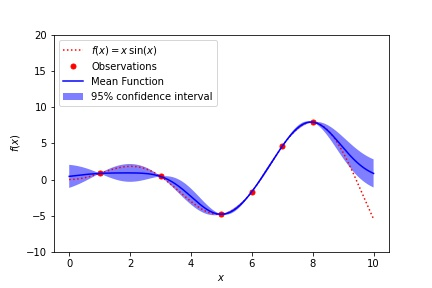
\includegraphics[scale=0.6]{RBF.jpg}
  \caption{SE Kernel with $l=1.0$}
  \label{fig:SE}
\end{figure}
\begin{figure}
\centering
  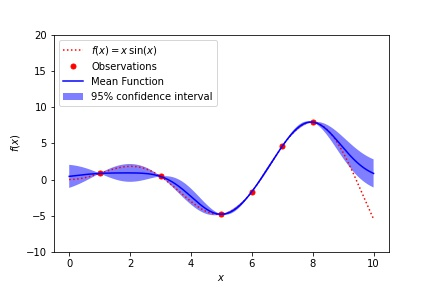
\includegraphics[scale=0.6]{RQ.jpg}
  \caption{RQ Kernel with $l = 1.0$ and $\alpha = 1e+05$}
  \label{fig:RQ}
\end{figure}
\begin{figure}
\centering
  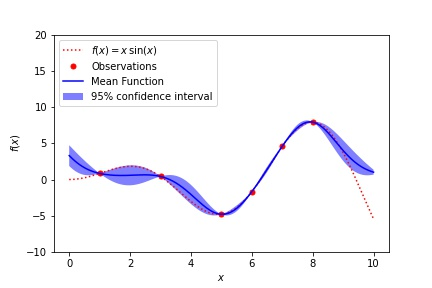
\includegraphics[scale=0.6]{Per.jpg}
  \caption{Periodic Kernel with $l = 0.6$ and $p = 9.0$}
  \label{fig:Per}
\end{figure}
\begin{figure}
\centering
  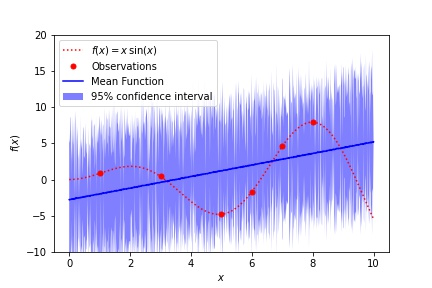
\includegraphics[scale=0.6]{Lin.jpg}
  \caption{Linear Kernel with $c = 0$ and $\sigma_{b} = 1.0$}
  \label{fig:Lin}
\end{figure}

%\section{Conclusion}
%``I always thought something was fundamentally wrong with the universe'' %\citep{adams1995hitchhiker}
%\bibliographystyle{plain}
%\bibliography{references}
\end{document}
